\documentclass{standalone}
\usepackage{tikz}
\usepackage{amsmath,amssymb}
\usetikzlibrary{arrows.meta,positioning,shapes,calc}
\begin{document}
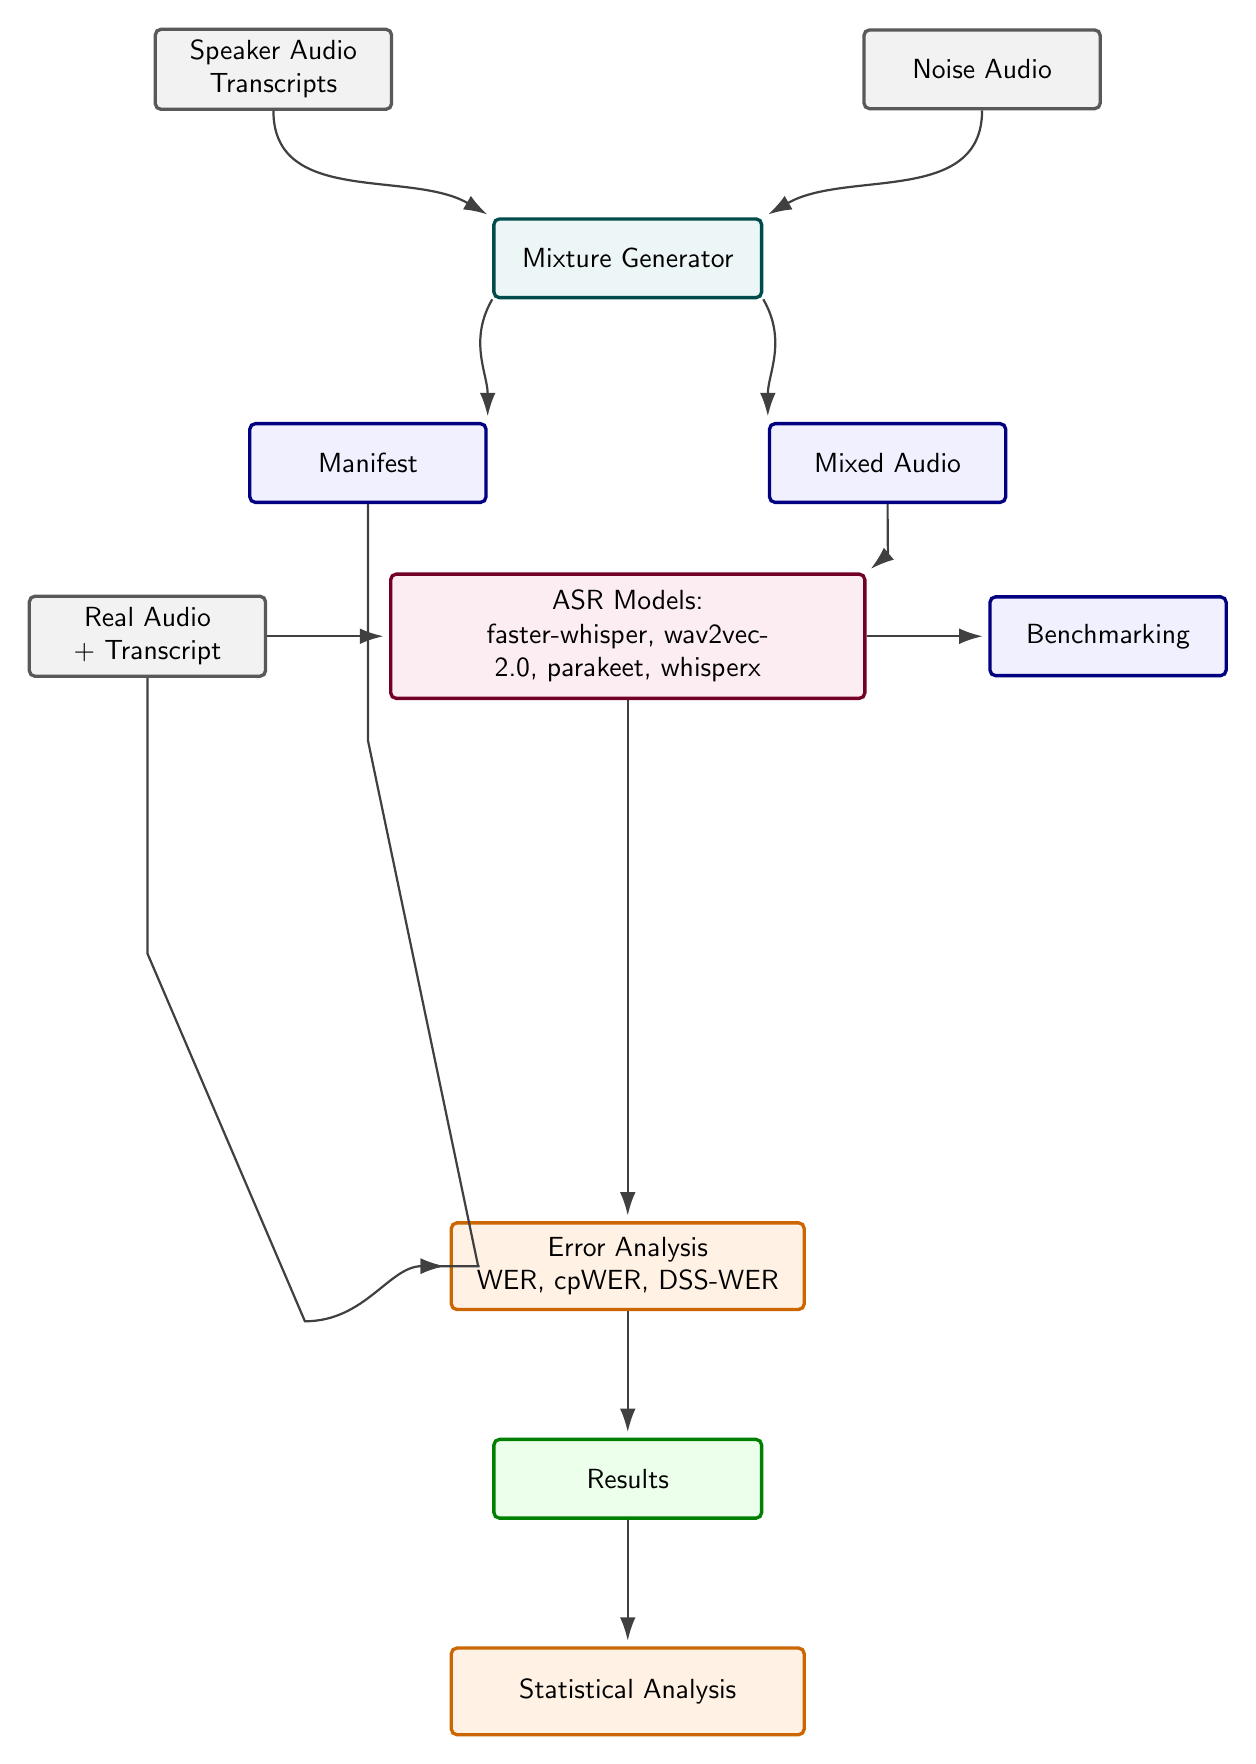
\begin{tikzpicture}[font=\sffamily, >=Latex, every node/.style={align=center}, line/.style={-{Latex[length=3mm,width=2mm]}, thick, draw=black!75}]

% styles
\tikzset{
  block/.style={rectangle, rounded corners=2pt, draw=blue!50!black, very thick, minimum height=10mm, minimum width=30mm, fill=blue!6, inner sep=4pt},
  process/.style={rectangle, rounded corners=2pt, draw=teal!60!black, very thick, minimum height=10mm, minimum width=34mm, fill=teal!7, inner sep=4pt},
  model/.style={rectangle, rounded corners=2pt, draw=purple!60!black, very thick, minimum height=14mm, text width=56mm, fill=purple!7, inner sep=6pt},
  analysis/.style={rectangle, rounded corners=2pt, draw=orange!80!black, very thick, minimum height=11mm, text width=42mm, fill=orange!10, inner sep=4pt},
  result/.style={rectangle, rounded corners=2pt, draw=green!50!black, very thick, minimum height=10mm, minimum width=34mm, fill=green!8, inner sep=4pt},
  io/.style={rectangle, rounded corners=2pt, draw=gray!70!black, very thick, minimum height=10mm, minimum width=30mm, fill=gray!10, inner sep=4pt}
}

% Absolute-positioned nodes to avoid overlaps
\node[io] (A) at (0,0) {Speaker Audio\\Transcripts};
\node[io] (C) at (9,0) {Noise Audio};

\node[process] (B) at (4.5,-2.4) {Mixture Generator};

\node[block] (D) at (1.2,-5) {Manifest};
\node[block] (E) at (7.8,-5) {Mixed Audio};

\node[model] (F) at (4.5,-7.2) {ASR Models:\\faster-whisper, wav2vec-2.0, parakeet, whisperx};

\node[io] (M) at (-1.6,-7.2) {Real Audio\\+ Transcript};
\node[block] (L) at (10.6,-7.2) {Benchmarking};

\node[analysis] (J) at (4.5,-15.2) {Error Analysis\\WER, cpWER, DSS-WER};
\node[result] (K) at (4.5,-17.9) {Results};
\node[analysis] (N) at (4.5,-20.6) {Statistical Analysis};

% Routing lines with explicit anchors and bends; shorten slightly to avoid touching borders
\draw[line,shorten >=2pt] (A.south) to[out=-90,in=150] (B.north west);
\draw[line,shorten >=2pt] (C.south) to[out=-90,in=30] (B.north east);
\draw[line,shorten >=2pt] (B.south west) to[out=-120,in=90] (D.north east);
\draw[line,shorten >=2pt] (B.south east) to[out=-60,in=90] (E.north west);
\draw[line,shorten >=2pt] (E.south) to[out=-90,in=40] (F.north east);
\draw[line,shorten >=2pt] (M.east) to[out=0,in=180] (F.west);

% connector coordinates to avoid overlapping the ASR box
% approach coordinates left of Error Analysis (different heights)
\coordinate (cD) at (2.6,-15.2);
\coordinate (cM) at (0.4,-15.9);

% Route manifest down then horizontally, then approach Error Analysis from left (upper)
\draw[line,shorten >=2pt] (D.south) -- ++(0,-3.0) -- (2.6,-15.2) to[out=0,in=180] (J.west);

% Route real-audio down then horizontally, then approach Error Analysis from left (lower)
\draw[line,shorten >=2pt] (M.south) -- ++(0,-3.5) -- (0.4,-15.9) to[out=0,in=180] (J.west);

\draw[line,shorten >=2pt] (F.south) -- (J.north);
\draw[line,shorten >=2pt] (F.east) to[out=0,in=180] (L.west);
\draw[line,shorten >=2pt] (J) -- (K);
\draw[line,shorten >=2pt] (K) -- (N);

\end{tikzpicture}
\end{document}
